\documentclass[12pt]{article}
\usepackage{graphicx}
  \graphicspath{ {./img/} }
\usepackage[figurename=Obr.]{caption}
\usepackage{multirow}
\usepackage{enumitem}
\usepackage{array}
\usepackage{geometry}
  \geometry{
  a4paper,
  top=25mm,
  left=20mm,
  right=20mm
}

\begin{document}
  \begin{titlepage}
    \begin{center}
      
\includegraphics[scale=0.1]{logo_cz}
    \end{center}
    \begin{center}
      \vspace{1.5cm}
      {\Large Projekt} \\
      \vspace{0.5cm}
      \textbf{\Large UART - přijímací část} \\
      \vspace{1.5cm}
      {\large INC - Návrh číslicových systémů} \\
      \vspace{0.5cm}
      {\large 2020/2021} \\
      \vfill
      Machyňák Augustin \hfill xmachy02 \hfill Květen 2021
    \end{center}
  \end{titlepage}

\newpage

\section{Architektura navrženého obvodu}
\begin{center}
  \begin{figure}[h!]
    \hfill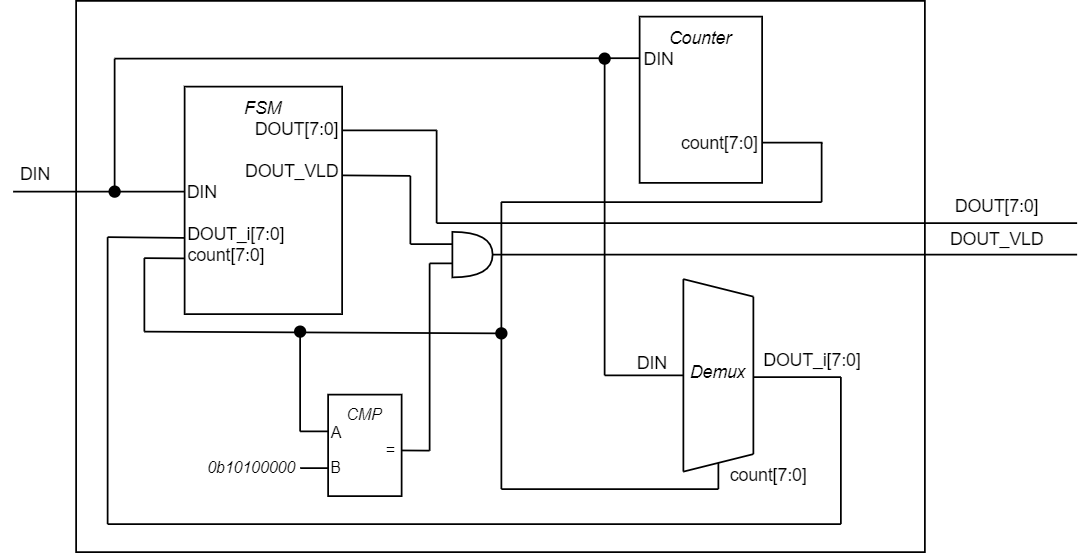
\includegraphics[scale=0.4]{rtl}\hspace*{\fill}
    \caption{\textit{Schéma obvodu}}
  \end{figure}
\end{center}

\subsection{Popis funkce}
  Obvod využívá stavového automatu, který mění stavy na základě hodnoty čítače
  a DIN. Jakmile čítač bude mít hodnotu:
  \begin{itemize}
    \item násobku 16 + 8 (24, 40, 56...) - příslušný bit DOUT je nastaven na
    hodnotu vstupu DIN.
    \item 160 - DOUT\_VLD je nastaven do log. 1 na 1 clk
  \end{itemize}
\newpage

\section{Návrh automatu (Finite State Machine)}
\begin{center}
  \begin{figure}[h!]
    \hfill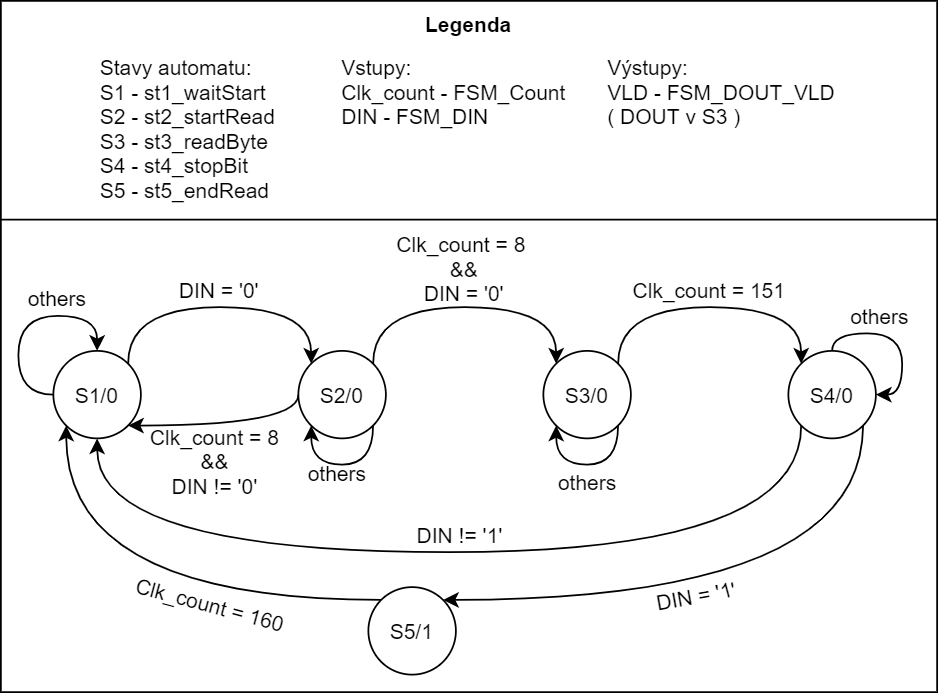
\includegraphics[scale=0.5]{fsm}\hspace*{\fill}
    \caption{\textit{Schéma automatu}}
  \end{figure}
\end{center}

\subsection{Popis funkce}
  Stavový automat přechází mezi stavy na základě hodnot DIN a Clk\_count. 
  Jakmile klesne hodnota DIN na log.0, tak přechází do stavu S2 a zároveň
  začne počítat čítač - Clk\_count. \\
  Po 8 clk periodách se přečte hodnota DIN (start bit) a pokud je log.0, 
  tak přechází do stavu S3.
  Ve stavu S3 se přečte přenesené slovo (1 bit každých 16 clk cyklů) a následně
  přechází do stavu S4, kde proběhne kontrola stop bitu.
  Pokud vše proběhlo v pořádku, tak ve stavu S5 je nastaveno DOUT\_VLD do log.1
  na 1 clk periodu a následně přechází zpět do stavu S1, kde čeká na přenos dalšího
  slova.

\newpage
\section{Simulace}
\begin{center}
  \begin{figure}[h!]
    \hfill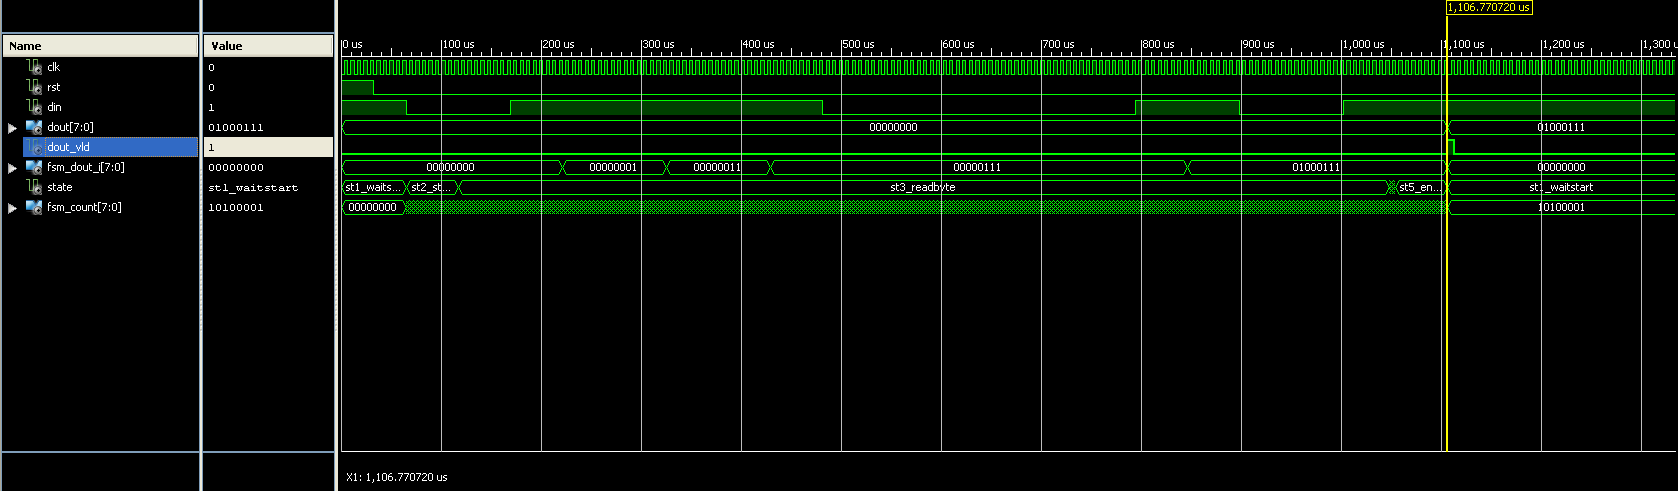
\includegraphics[scale=0.38]{simout}\hspace*{\fill}
    \caption{\textit{Snímek simulace při přenosu 1 slova}}
  \end{figure}
\end{center}

\end{document}